\chapter{Dados}
\label{chap:dados}

Este capítulo descreve as bases de dados utilizadas na dissertação e apresenta
uma análise exploratória das principais variáveis de interesse. O objetivo é
caracterizar as propriedades estatísticas do prêmio de risco de volatilidade do
Bitcoin, bem como sua relação preliminar com medidas de volatilidade e retornos
do ativo, fornecendo motivação empírica para as análises econométricas e
preditivas desenvolvidas nos capítulos subsequentes.

A análise conduzida neste capítulo possui caráter estritamente descritivo e
exploratório, não implicando inferências causais. Ainda assim, ela é fundamental
para compreender a dinâmica temporal, a distribuição estatística e a
heterogeneidade do prêmio de risco de volatilidade ao longo da amostra,
estabelecendo o pano de fundo empírico para os modelos apresentados nos
Capítulos~\ref{chap:metodologia} e~\ref{chap:resultados_ols}.

% =========================================================
\section{Descrição das variáveis e estatísticas descritivas}
\label{sec:estatisticas_descritivas}

A base de dados utilizada é composta por observações diárias do mercado de
Bitcoin, combinando informações do mercado à vista e do mercado de opções.
Especificamente, são considerados: (i) retornos do Bitcoin no mercado à vista;
(ii) volatilidade realizada construída a partir desses retornos; (iii)
volatilidade implícita extraída do mercado de opções negociadas na plataforma
Deribit; e (iv) o prêmio de risco de volatilidade do Bitcoin (BVRP).

As medidas de volatilidade implícita e realizada são construídas em janelas
móveis de 30 dias, de modo a garantir comparabilidade temporal entre ambas,
alinhando-se às práticas de mercado e à literatura empírica sobre prêmio de
risco de volatilidade. A volatilidade implícita a 30 dias é consistente com o
horizonte do índice DVOL da Deribit, enquanto a volatilidade realizada é
anualizada considerando a negociação contínua do mercado de Bitcoin.

A Tabela~\ref{tab:estatisticas_cap3} apresenta estatísticas descritivas das
principais variáveis empregadas na análise empírica, incluindo média, desvio
padrão, valores mínimo e máximo. Observa-se que tanto a volatilidade implícita
quanto a volatilidade realizada exibem elevada variabilidade, refletindo a
natureza altamente volátil do mercado de criptoativos. O prêmio de risco de
volatilidade apresenta média positiva ao longo da amostra, consistente com a
existência de uma compensação exigida pelos investidores para assumir risco de
volatilidade no mercado de opções de Bitcoin.

  \begin{table}[H]
\centering
\caption{Estatísticas descritivas das variáveis principais e retornos futuros}
\label{tab:estatisticas_cap3}
\begin{tabular}{lcccc}
\toprule
 & Média & Desvio-padrão & Mínimo & Máximo \\
\midrule
IV30D & 53.029358 & 9.764681 & 32.380000 & 83.020000 \\
RV30D & 47.674015 & 14.853184 & 16.756112 & 87.430263 \\
BVRP (IV30D - RV30D) & 5.355343 & 11.587143 & -32.405652 & 28.355131 \\
Retorno futuro 1D & 0.002671 & 0.026530 & -0.083902 & 0.229507 \\
Retorno futuro 5D & 0.012609 & 0.056642 & -0.164158 & 0.230331 \\
Retorno futuro 20D & 0.047105 & 0.119952 & -0.169503 & 0.442889 \\
\bottomrule
\end{tabular}
\end{table}


}{}

% =========================================================
\section{Séries temporais}
\label{sec:series_temporais}

A análise das séries temporais das variáveis de interesse permite avaliar a
dinâmica da volatilidade e do prêmio de risco ao longo do tempo, bem como
identificar episódios de persistência e mudanças de comportamento associados a
eventos relevantes do mercado de criptoativos. A
Figura~\ref{fig:vrp_timeseries} apresenta a evolução temporal do prêmio de risco
de volatilidade do Bitcoin ao longo da amostra.

\IfFileExists{figs/vrp_timeseries.png}{
\begin{figure}[H]
    \centering
    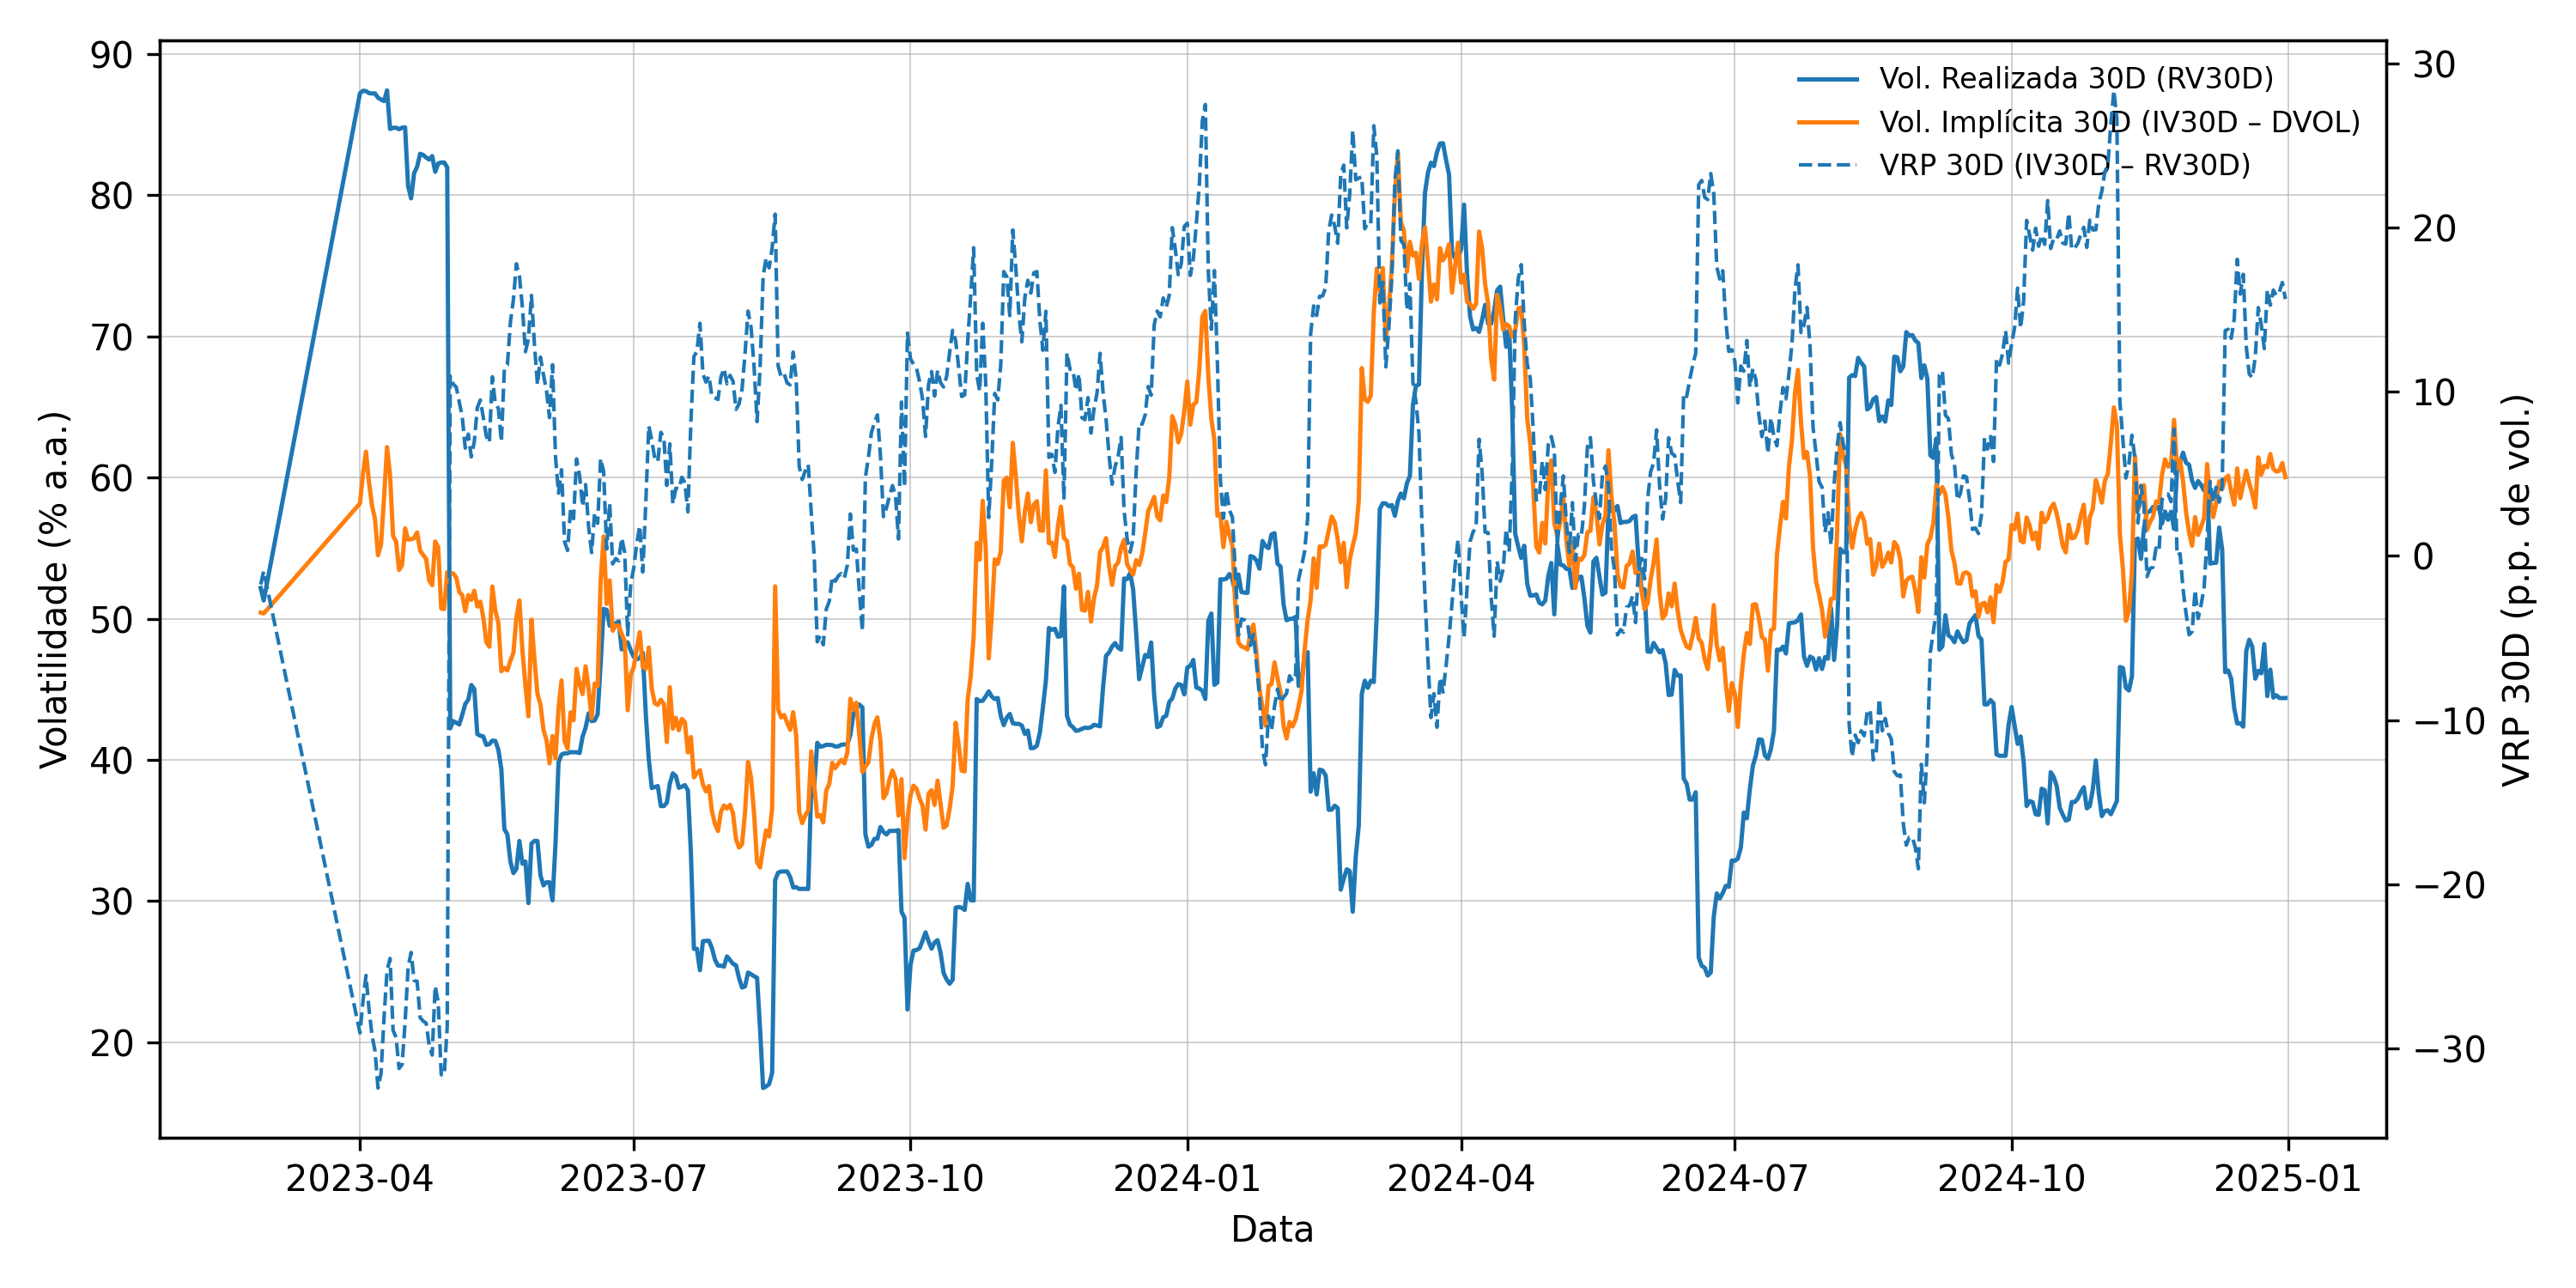
\includegraphics[width=0.9\linewidth]{figs/vrp_timeseries.png}
    \caption{Evolução temporal do prêmio de risco de volatilidade do Bitcoin (BVRP)}
    \label{fig:vrp_timeseries}
\end{figure}
}{}

A inspeção visual da série evidencia períodos recorrentes de elevação do prêmio
de risco de volatilidade, frequentemente associados a episódios de estresse no
mercado, como choques macroeconômicos globais, eventos regulatórios relevantes e
fases de forte desalavancagem. Observa-se também a presença de persistência
temporal, sugerindo que o BVRP não se comporta como um processo puramente
aleatório, mas apresenta dinâmica própria ao longo do tempo.

% =========================================================
\section{Distribuições empíricas}
\label{sec:distribuicoes}

A análise das distribuições empíricas fornece evidências adicionais sobre as
propriedades estatísticas das variáveis consideradas. A
Figura~\ref{fig:vrp_hist} apresenta o histograma do prêmio de risco de
volatilidade do Bitcoin, juntamente com uma estimativa de densidade por kernel.

\IfFileExists{figs/vrp_histogram_kde.png}{
\begin{figure}[H]
    \centering
    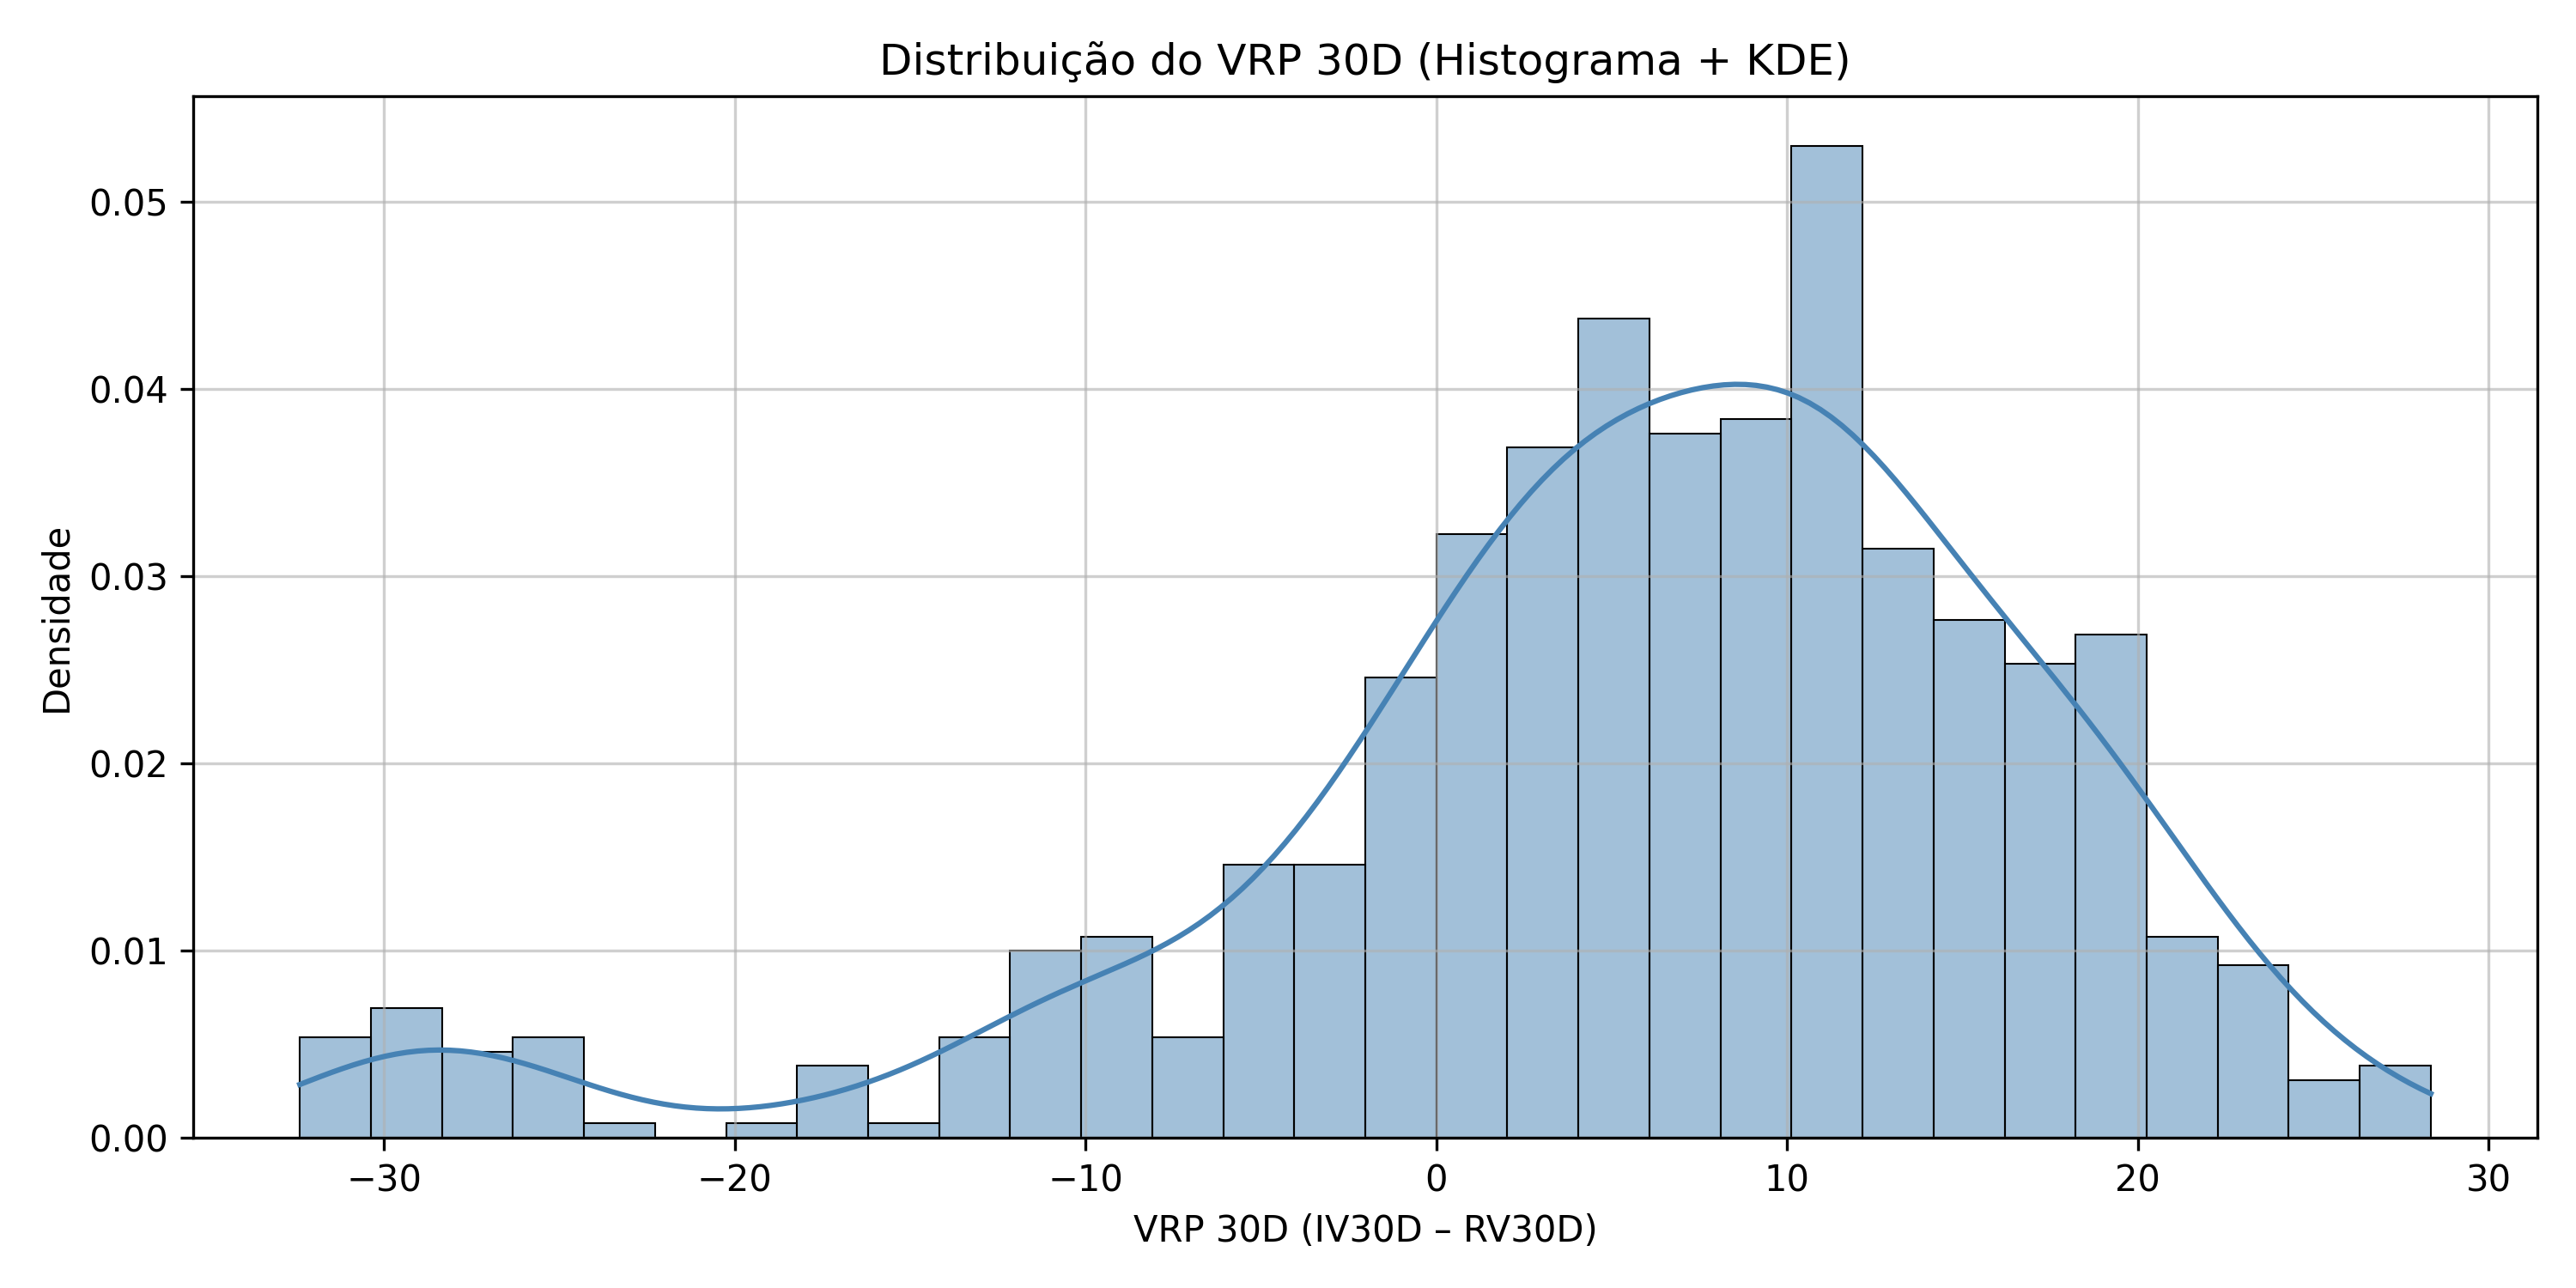
\includegraphics[width=0.75\linewidth]{figs/vrp_histogram_kde.png}
    \caption{Distribuição empírica do prêmio de risco de volatilidade do Bitcoin}
    \label{fig:vrp_hist}
\end{figure}
}{}

Observa-se que a distribuição do prêmio de risco de volatilidade apresenta
assimetria e caudas pesadas, afastando-se da hipótese de normalidade. Essas
características são amplamente documentadas na literatura empírica sobre
mercados financeiros e tornam-se ainda mais pronunciadas no contexto de
criptoativos, nos quais eventos extremos ocorrem com maior frequência. Tal
evidência reforça a necessidade de abordagens econométricas robustas e motiva o
uso de metodologias mais flexíveis nos capítulos subsequentes.

% =========================================================
\section{Análise por regimes e subperíodos}
\label{sec:regimes}

Com o objetivo de avaliar a heterogeneidade temporal do prêmio de risco de
volatilidade, a amostra é segmentada em subperíodos e regimes associados a
diferentes níveis de volatilidade. A
Figura~\ref{fig:vrp_boxplot} apresenta a distribuição do BVRP ao longo do tempo
por meio de boxplots.

\IfFileExists{figs/vrp_boxplot.png}{
\begin{figure}[H]
    \centering
    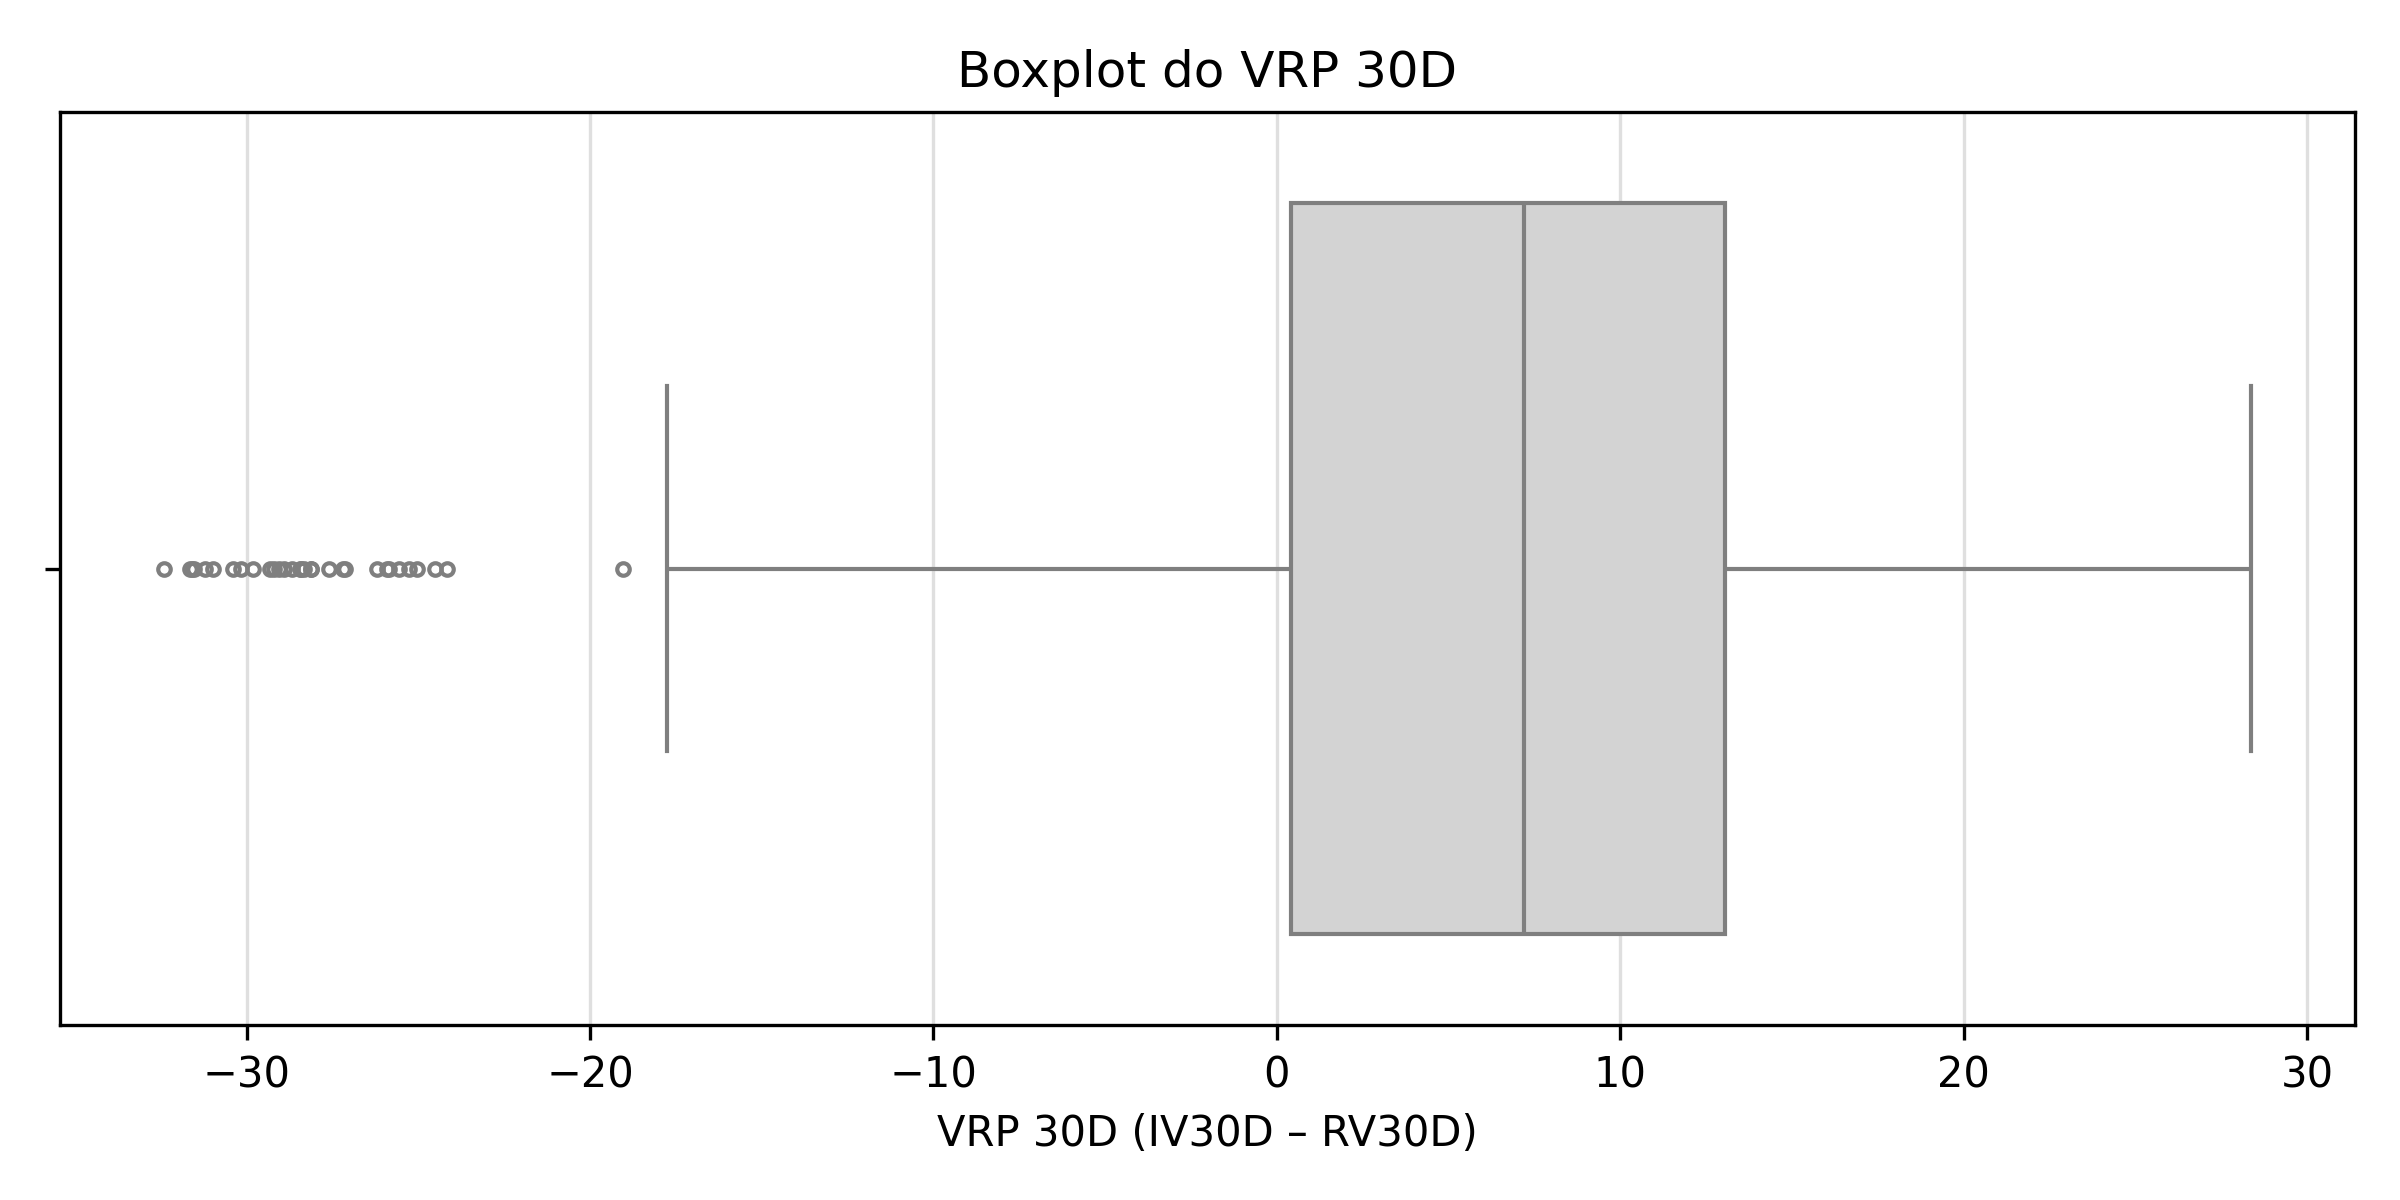
\includegraphics[width=0.85\linewidth]{figs/vrp_boxplot.png}
    \caption{Distribuição do prêmio de risco de volatilidade do Bitcoin por
    subperíodos e regimes}
    \label{fig:vrp_boxplot}
\end{figure}
}{}

Os resultados indicam que o prêmio de risco de volatilidade não é homogêneo ao
longo do tempo, assumindo valores mais elevados em períodos caracterizados por
maior incerteza e volatilidade do mercado. Essa evidência sugere que modelos com
parâmetros constantes podem ser insuficientes para capturar plenamente a
dinâmica do BVRP, justificando a adoção de abordagens que permitam variação
temporal e efeitos de regime nos capítulos subsequentes.

% =========================================================
\section{Relações iniciais entre prêmio de risco de volatilidade e retornos}
\label{sec:vrp_retornos}

Por fim, são examinadas relações exploratórias entre o prêmio de risco de
volatilidade do Bitcoin e os retornos futuros do ativo em diferentes horizontes
temporais. A
Figura~\ref{fig:vrp_ret_20d} apresenta o gráfico de dispersão entre o BVRP
observado no tempo $t$ e o retorno futuro acumulado do Bitcoin no horizonte de
20 dias, juntamente com uma reta de tendência linear.

\IfFileExists{figs/vrp_vs_return_20d.png}{
\begin{figure}[H]
    \centering
    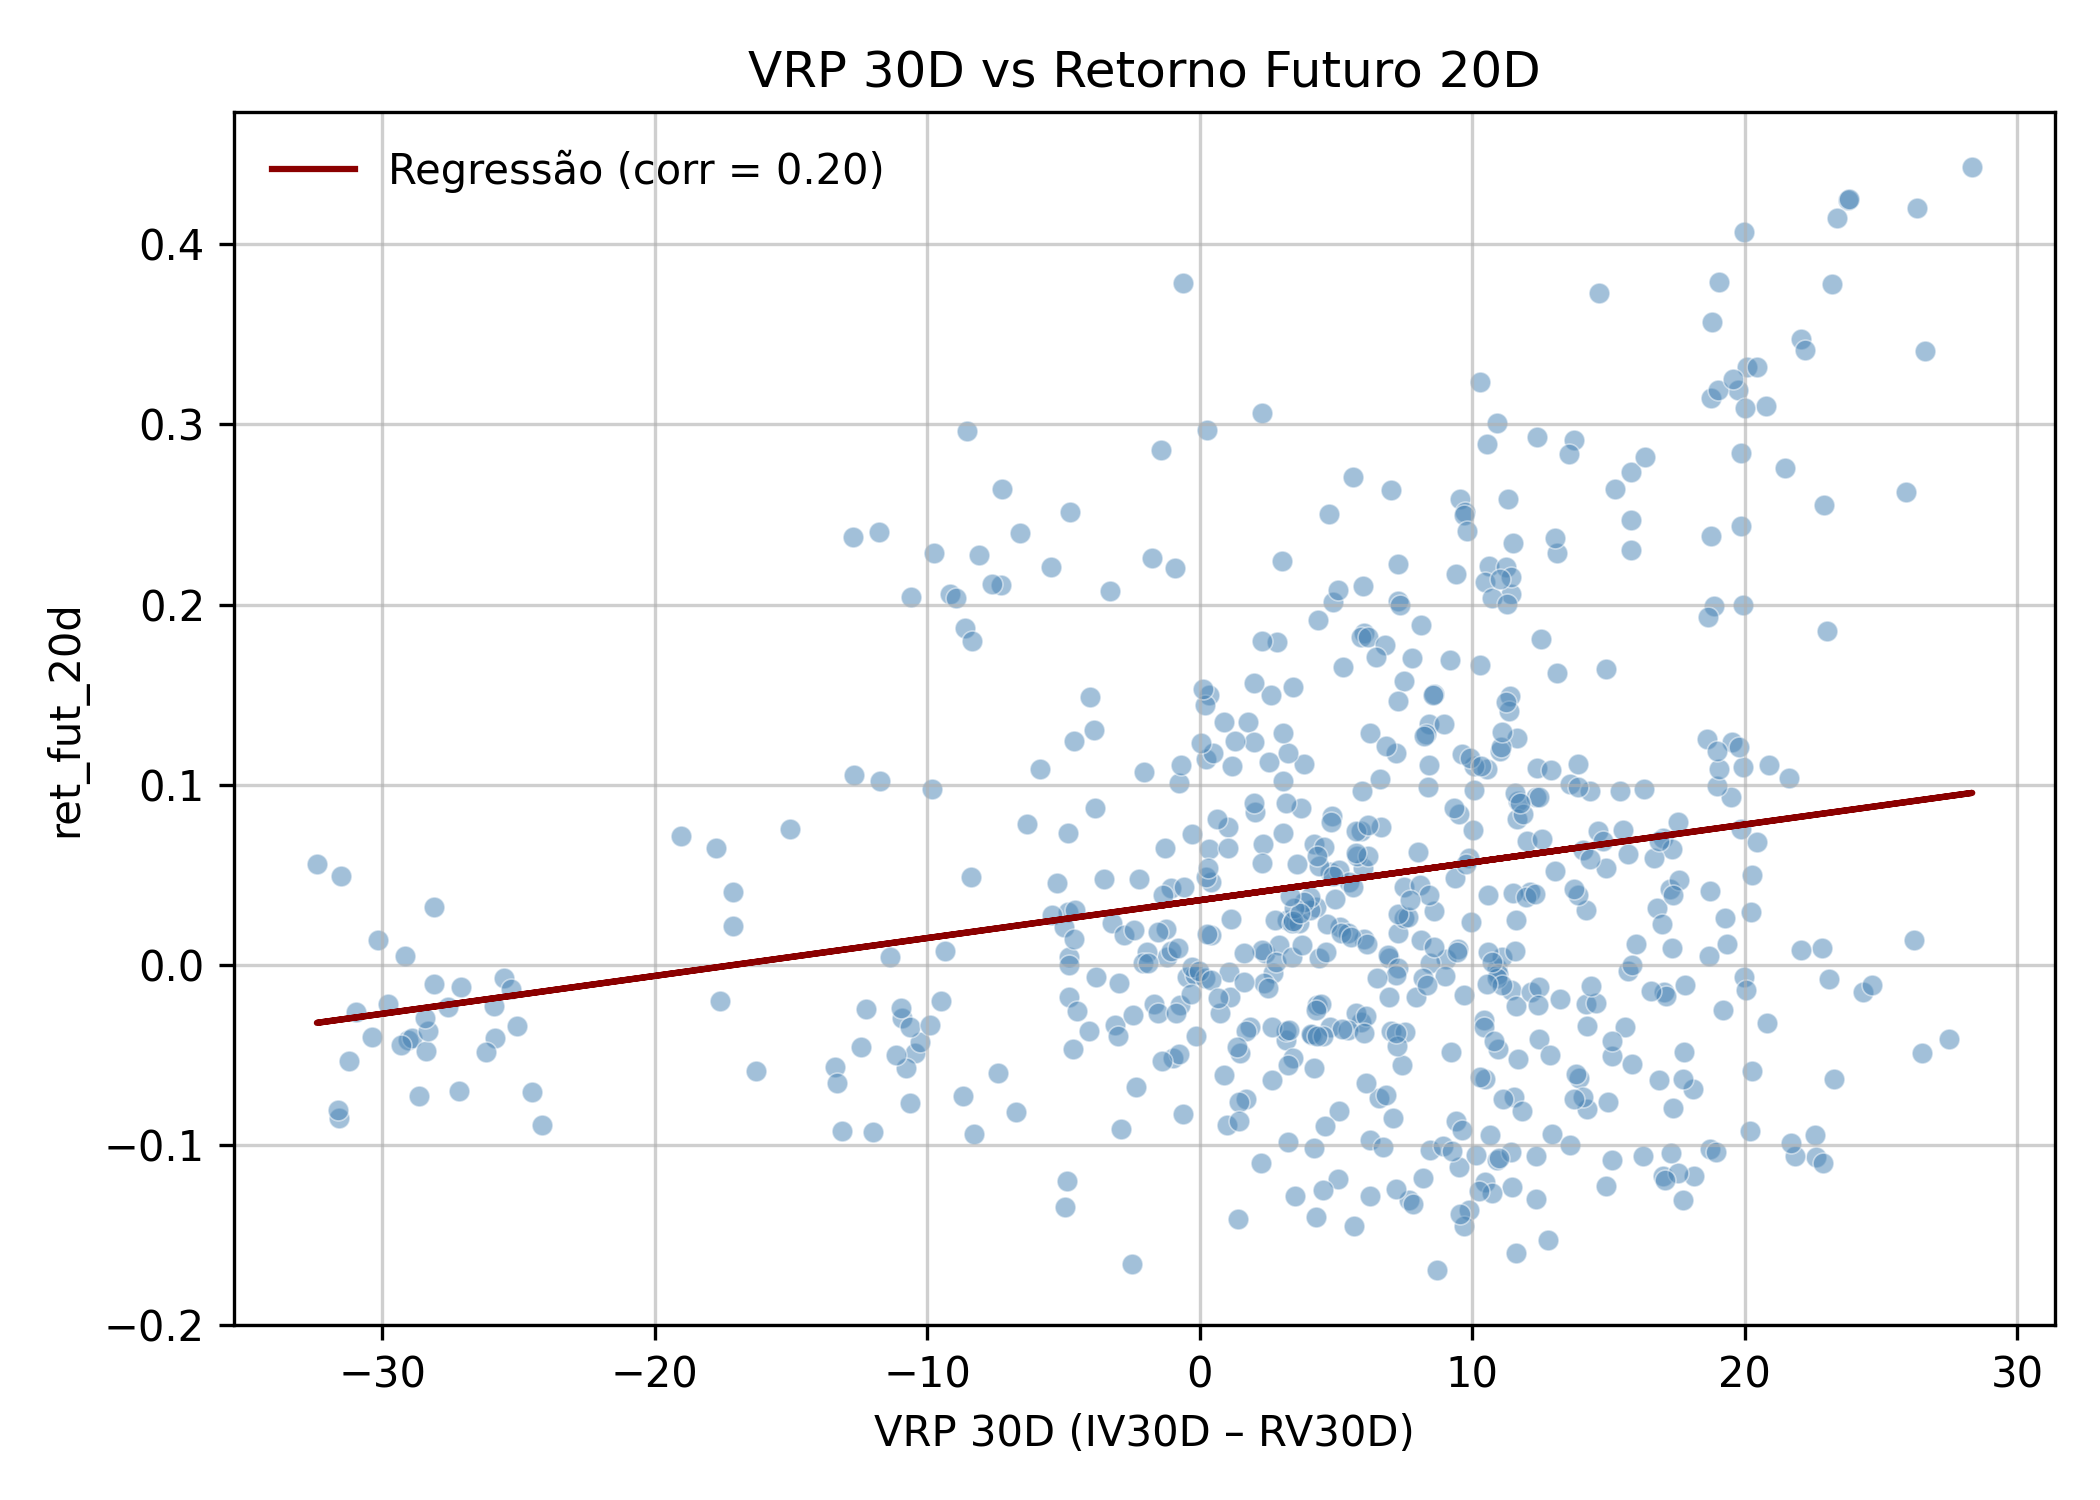
\includegraphics[width=0.75\linewidth]{figs/vrp_vs_return_20d.png}
    \caption{Relação exploratória entre o prêmio de risco de volatilidade e os
    retornos futuros do Bitcoin (h = 20 dias)}
    \label{fig:vrp_ret_20d}
\end{figure}
}{}

A análise visual sugere a existência de uma relação média entre o prêmio de risco
de volatilidade e os retornos futuros, ainda que acompanhada por elevada
dispersão. Essas evidências possuem caráter estritamente descritivo e não
implicam relações causais. Ainda assim, fornecem motivação econômica clara para
os testes econométricos desenvolvidos no Capítulo~\ref{chap:resultados_ols}, nos
quais o conteúdo informacional do prêmio de risco de volatilidade é avaliado de
forma rigorosa por meio de modelos lineares estimados por mínimos quadrados
ordinários.
